\part{Python programming II}
\section{Scientific computing}
\subsection{Introduction}
\begin{frame}[label=contents_prog2]
  \frametitle{Today's outline}
  \mode<beamer>{
    \only<1>{\tableofcontents}
  }
  \only<2>{\tableofcontents[currentsection]}
\end{frame}
% \begin{frame}[label=contents_prog2]
%   \frametitle{Today's outline}
%   \mode<beamer>{
%     \only<1>{
%       \begin{columns}
%         \column{0.5\textwidth}
%           \tableofcontents[sections={1-3}]
%         \column{0.5\textwidth}
%           \tableofcontents[sections={4-8}]
%       \end{columns}}
%   }
%   \only<2>{
%     \begin{columns}
%       \column{0.5\textwidth}
%         \tableofcontents[sections={1-3},currentsection]
%       \column{0.5\textwidth}
%         \tableofcontents[sections={4-8},currentsection]
%     \end{columns}
%     }
% \end{frame}

%% NUMPY
\subsection{Introduction to NumPy}
\begin{frame}[fragile]
  \frametitle{Introduction to NumPy (1)}
  NumPy is a powerful library for numerical computing in Python. It introduces the multidimensional array (\lstinline|ndarray|) data structure which is central to numerical computing tasks. To start using NumPy, you need to import it first:
  \begin{lstlisting}[language=Python, numbers=none]
>>> import numpy as np
  \end{lstlisting}\pause
  Creating arrays from Python lists and accessing elements:
  \begin{lstlisting}[language=Python, numbers=none]
>>> arr = np.array([1, 2, 3, 4, 5])
>>> arr[0]
1
  \end{lstlisting}\pause
  Create arrays with predetermined values:
  \begin{lstlisting}[language=Python, numbers=none]
>>> np.zeros(5)  # Creates an array of five zeros
>>> np.ones((3, 3))  # Creates a 3x3 array of ones - note that the input argument is a tuple
  \end{lstlisting}
\end{frame}

\begin{frame}[fragile]
  \frametitle{Introduction to NumPy (2)}
  Useful array creation functions:
  \begin{lstlisting}[language=Python, numbers=none]
>>> arr  = np.arange(0, 10, 2)  # Creates an array with values from 0 to 10, step 2
>>> arr2 = np.linspace(0, 1, 5) # Creates an array with 5 values evenly spaced between 0 and 1
>>> arr3 = np.logspace(-3,2,6)  # Creates an array spaced evenly on a logscale
  \end{lstlisting}\pause

  Array operations:
  \begin{lstlisting}[language=Python, numbers=none]
>>> arr * 2  # Multiplies every element by 2
>>> arr + np.array([5, 4, 3, 2, 1])  # Element-wise addition
  \end{lstlisting}\pause
  
  Inspecting your array:
  \begin{lstlisting}[language=Python, numbers=none]
>>> arr.shape  # Returns the dimensions of the array (tuple)
>>> arr.shape[0] # Returns the number of rows ([1] for columns)
>>> len(arr)  # Returns the size of the first dimension
>>> arr.size # Returns the total number of elements in arr
  \end{lstlisting}
\end{frame}

\begin{frame}[fragile]
  \frametitle{Introduction to NumPy (3)}
  Zeros- or ones-filled arrays:
  \begin{lstlisting}[language=Python, numbers=none]
>>> many_zeros = np.zeros_like(arr) # Array with zeros of size like arr, also: np.zeros
>>> just_ones  = np.ones((2,4))     # Create array with ones of size (2,4), also: np.ones_like
>>> identity   = np.eye((3,3))      # Identity matrix (zeros with ones on the main diagonal)
    \end{lstlisting}\pause
      
    Or random numbers, useful for e.g. stochastic simulations. Note that these are NumPy intrinsic methods, and differ from the ones in the \lstinline|random| module.
    \begin{lstlisting}[language=Python, numbers=none]
>>> np.random.rand() # Single random floating point number [0,1)
0.11879317099184983

>>> np.random.rand(2,3)
array([[0.36482694, 0.47204049, 0.20908193],
       [0.76626339, 0.64075302, 0.82440279]])

>>> np.random.randint(1,10,5) # 5 random integers from 1 (inclusive) until 10 (exclusive)
array([9, 1, 6, 4, 6])
        \end{lstlisting}\pause
\end{frame}

%% MATH WITH NUMPY
\subsection{Math with NumPy}
\begin{frame}[fragile]
  \frametitle{Math with NumPy (1)}
  NumPy provides a rich set of functions to perform mathematical operations on arrays. Let's explore some categories of these operations.
  \begin{itemize}
    \item Linear Algebra:
    \begin{lstlisting}[language=Python, numbers=none]
>>> np.dot(arr, arr)     # Dot product (alternative: arr @ arr)
>>> np.linalg.norm(arr)  # Euclidean norm (L2 norm)
    \end{lstlisting}\pause
    
    \item Trigonometric Functions:
  \begin{lstlisting}[language=Python, numbers=none]
>>> np.sin(arr)  # Sine of each element
>>> np.cos(arr)  # Cosine of each element
  \end{lstlisting}
  
  \item Statistical functions to analyze data:
  \begin{lstlisting}[language=Python, numbers=none]
>>> np.mean(arr)  # Mean value of the array elements
>>> np.std(arr)   # Standard deviation of the array elements
  \end{lstlisting}\pause
\end{itemize}
\end{frame}


{\nologo
\begin{frame}[fragile]
  \frametitle{Math with NumPy (2)}
  \textbf{Table: Useful NumPy Functions for Beginners}

  \begin{tabular}{l|l}
  Function & Description \\
  \hline
  \lstinline$np.array$ & Create a NumPy array \\
  \lstinline$np.zeros$ & Create an array filled with zeros \\
  \lstinline$np.ones$ & Create an array filled with ones \\
  \lstinline$np.arange$ & Create an array with evenly spaced values \\
  \lstinline$np.linspace$ & Create an array with a specified number of evenly spaced values \\
  \lstinline$np.sin$ & Sine function \\
  \lstinline$np.cos$ & Cosine function \\
  \lstinline$np.tan$ & Tangent function \\
  \lstinline$np.exp$ & Exponential function \\
  \lstinline$np.log$ & Natural logarithm \\
  \lstinline$np.sqrt$ & Square root function \\
  \lstinline$np.dot$ & Dot product of two arrays \\
  \lstinline$np.linalg.norm$ & Calculate the norm of an array \\
  \lstinline$np.mean$ & Calculate the mean of an array \\
  \lstinline$np.std$ & Calculate the standard deviation of an array \\
  \end{tabular}
\end{frame}
}

%% ARRAY OPERATIONS
\subsection{Array operations}
\begin{frame}[fragile]
  \frametitle{Array operations (1)}
  In Python, NumPy ndarrays enable efficient operations on arrays, particularly mathematical operations associated with linear algebra. Let's look at how we can create and manipulate matrices using NumPy ndarrays:
  \begin{itemize}
    \item Manually creating matrices (2D ndarrays):
    \begin{lstlisting}[language=Python, numbers=none]
>>> import numpy as np
>>> matrix = np.array([[1, 2], 
                      [3, 4]]) # Matrices are arrays of arrays(rows)
    \end{lstlisting}\pause

    \item Reshaping, slicing and modifying matrices (try for yourself and print each new result):
    \begin{lstlisting}[language=Python, numbers=none]
>>> mat = np.arange(25).reshape(5,5)
>>> col = mat[:,2]  # Get column index 2
>>> row = mat[3,:]  # Get row index 3
>>> sub = mat[1:4,1:4] # Save submatrix
>>> mat[1,:] = row  # Replace row index 1 by 'row'
>>> mat[mat>5] = -1 # Conditional slicing/update of values
    \end{lstlisting}
  \end{itemize}
\end{frame}

\begin{frame}[fragile]
  \frametitle{Array operations (2)}
  The real power of NumPy lies in the vectorized computations:
  \begin{itemize}
    \item Omit loops, write computations in natural language
    \item Shorter code
    \item Much, much faster
  \end{itemize}
  \pause
  \begin{lstlisting}
import numpy as np
import time

start = time.time()
x = np.linspace(0,2*np.pi,10000000)
y = np.exp(-x) * (2+np.sin(2*np.pi*x))
total_time = time.time() - start

print(f'{total_time = }')
  \end{lstlisting}
  \begin{lstlisting}[style=PyOutput]
total_time = 0.35589122772216797
  \end{lstlisting}
\end{frame}


\begin{frame}[fragile]
  \frametitle{Array operations (3)}
  If you do need to iterate over the elements:
  \begin{itemize}
    \item Think twice if you \emph{really} have to
    \item If the answer is still yes, you can use \lstinline|np.nditer| or \lstinline|np.ndenumerate|:
  \end{itemize}
  \pause
  \begin{columns}
    \column{0.5\textwidth}      
    \begin{lstlisting}
import numpy as np 

# A 2D array
data = np.array([[11,12,13], [14,15,16]])

# Loop over each element using nditer
for val in np.nditer(data):
    print(f"Value: {val}")

# Loop using ndenumerate (gives index + value)
for i,val in np.ndenumerate(data):
    print(f"Enumerate index {i} has value {val}; also {data[i]}")
    \end{lstlisting}
    \column{0.5\textwidth}
    \begin{lstlisting}[style=PyOutput]
Value: 11
Value: 12
Value: 13
Value: 14
Value: 15
Value: 16
Enumerate index (0, 0) has value 11; also 11
Enumerate index (0, 1) has value 12; also 12
Enumerate index (0, 2) has value 13; also 13
Enumerate index (1, 0) has value 14; also 14
Enumerate index (1, 1) has value 15; also 15
Enumerate index (1, 2) has value 16; also 16
    \end{lstlisting}
  \end{columns}
\end{frame}

{\nologo
\begin{frame}[fragile]
  \frametitle{Practice}
  Given a function $\displaystyle  f(x) = x^2+2x-4 $
  % \vskip-1em
  \begin{itemize}
   \item Create a large \lstinline|np.linspace| of $x\in[0,20]$ e.g. with 1M numbers
   \item Compute $f(x)$ iteratively (i.e. with a .loop)
   \item Compute $f(x)$ vectorized (i.e. using NumPy operations)
   \item Compare timings
  \end{itemize}
   \pause
   \begin{onlyenv}<beamer> 
    \begin{lstlisting}[basicstyle=\tiny\ttfamily]
import time

def f(x):
    return x**2+2*x-4

long_data = np.linspace(0,20,10_000_000)

start = time.time()
y1 = f(long_data)
print(f"The vectorized approach took {time.time()-start} seconds")

y2 = np.zeros_like(long_data)
start = time.time()
for i in range(len(long_data)):
    y2[i] = f(long_data[i])
print(f"The iterated approach took {time.time()-start} seconds")
    \end{lstlisting}
    \end{onlyenv}
 \end{frame}
}

\begin{frame}[fragile]
  \frametitle{Assignment of arrays by reference}
  Careful with assignment, default is a reference to the same object as observed with lists:
  \begin{lstlisting}[language=Python, numbers=none]
>>> arr = np.arange(0,10,1)
>>> print(arr)
[0 1 2 3 4 5 6 7 8 9]
>>> new_arr = arr 
>>> new_arr2 = arr.copy()
>>> new_arr[4] = 11
>>> print(new_arr)
[ 0  1  2  3 11  5  6  7  8  9]
>>> print(arr) # :mind_blown: we did not change this, did we?
[ 0  1  2  3 11  5  6  7  8  9]
  \end{lstlisting}\pause

  Saving and loading matrices:
  \begin{lstlisting}[language=Python, numbers=none]
>>> np.save('my_matrix.npy', matrix)  # Save the matrix to a file
>>> loaded_matrix = np.load('my_matrix.npy')  # Load the matrix from a file
  \end{lstlisting}
\end{frame}

% \begin{frame}[fragile]
%   \frametitle{Matrix Operations with NumPy ndarrays}
%   NumPy offers a rich set of functions to perform various matrix operations, essential in linear algebra. Let's explore some of them.\pause

%   Matrix Transposition and Inversion:
%   \begin{lstlisting}[language=Python, numbers=none]
% >>> np.transpose(matrix)  # Find the transpose of the matrix
% >>> np.linalg.inv(matrix)  # Find the inverse of the matrix
%   \end{lstlisting}\pause

%   Matrix Products and Dot Products:
%   \begin{lstlisting}[language=Python, numbers=none]
% >>> np.dot(matrix, matrix)  # Find the dot product
% >>> matrix @ matrix  # Alternative way to find the dot product
%   \end{lstlisting}
% \end{frame}

% \begin{frame}[fragile]
%   \frametitle{Advanced Linear Algebra with NumPy}
%   NumPy provides more advanced linear algebra operations that are fundamental in many scientific computations. Let's delve into some of these.\pause
  
%   Determinant and Rank of a Matrix:
%   \begin{lstlisting}[language=Python, numbers=none]
% >>> np.linalg.det(matrix)  # Find the determinant of the matrix
% >>> np.linalg.matrix_rank(matrix)  # Find the rank of the matrix
%   \end{lstlisting}\pause
  
%   Eigenvalues and Eigenvectors:
%   \begin{lstlisting}[language=Python, numbers=none]
% >>> np.linalg.eig(matrix)  # Find the eigenvalues and eigenvectors of the matrix
%   \end{lstlisting}
% \end{frame}


%% PLOTTING 
\section{Plotting with Matplotlib}
\subsection{Line plots}
\againframe<2>{contents_prog2}

\begin{frame}[fragile]
  \frametitle{Introduction to Matplotlib}
  Matplotlib is a Python library used widely for creating static, animated, and interactive visualizations. To start, we first import the \lstinline{pyplot} module from \lstinline{matplotlib}.\pause
  
  \begin{lstlisting}[language=Python]
import matplotlib.pyplot as plt
  \end{lstlisting}\pause
  
  \begin{columns}[T]
    \column{0.45\textwidth}
    Creating a simple line plot:

    \begin{lstlisting}[language=Python,firstnumber=2]
x = [1, 2, 3, 4, 5]
y = [2, 4, 1, 3, 7]
plt.plot(x, y)
plt.show()
  \end{lstlisting}\pause \vskip1em
  {\small In Jupyter Notebooks, use \lstinline|%matplotlib| to display figures in a separate window, or \lstinline|%matplotlib inline| to display in the notebook.}
    \column{0.45\textwidth}
  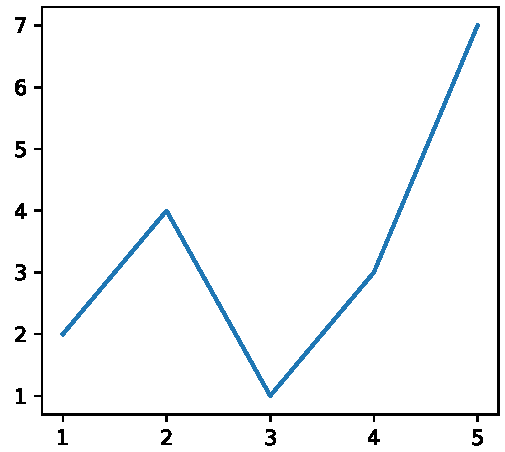
\includegraphics[width=0.7\textwidth]{intro_matplotlib.pdf}
\end{columns}
\end{frame}

\begin{frame}[fragile]
  \frametitle{Brushing up the graph}
  Adding multiple plots, axis labels and a legend:
  \begin{columns}
    \column{0.5\textwidth}
    \begin{lstlisting}[language=Python]
import matplotlib.pyplot as plt
import numpy as np

t = np.linspace(-2*np.pi, 2*np.pi,101)
y1 = 4*np.sin(t)/t + 2
y2 = np.sin(t)**2 - t/2 + 2

plt.plot(t,y1,label='Eqn 1')
plt.plot(t,y2,label='Eqn 2')
plt.xlabel('Time [s]')
plt.ylabel('Function value [-]')
plt.legend()
plt.grid()
plt.show()
    \end{lstlisting}\pause
    \column{0.5\textwidth}
      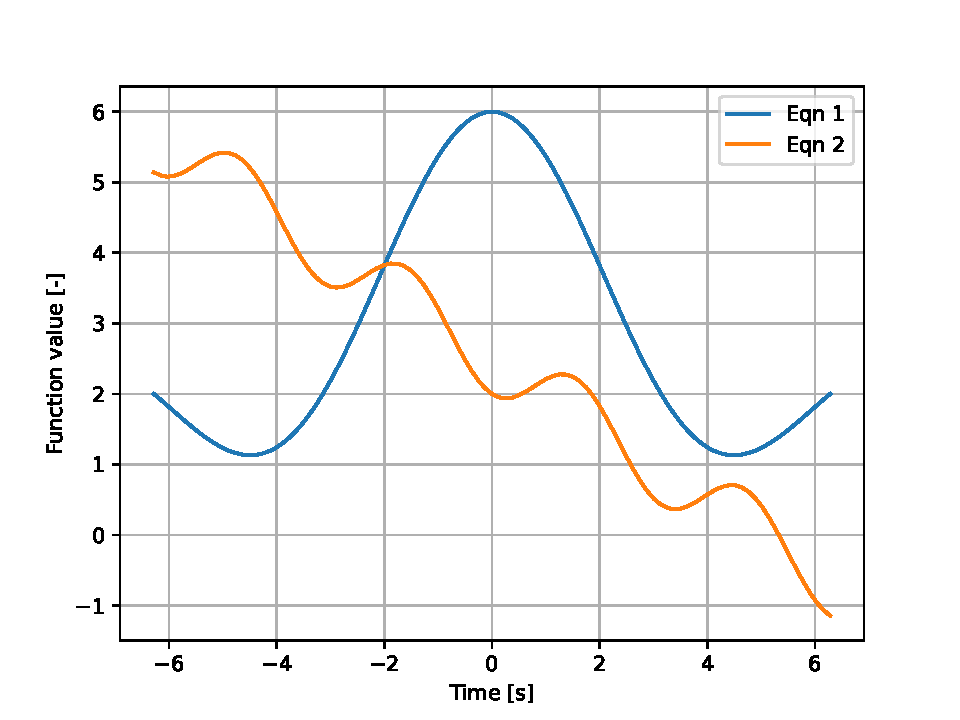
\includegraphics[width=\textwidth]{intro_matplotlib_2.pdf}
  \end{columns}
\end{frame}

\begin{frame}[fragile]
  \frametitle{Line plot styles}
  Changing markers, line styles:
  \begin{columns}
    \column{0.5\textwidth}
    \begin{lstlisting}[language=Python]
import matplotlib.pyplot as plt
import numpy as np

t = np.linspace(-10.0, 10.0, 20)
p = np.cos(np.pi * t/10) 
q = 1/(1+np.exp(-t)) - 0.5

plt.plot(t,p,'--x') # Dashed line, cross
plt.plot(t,q,'r-o') # Red, line, circles
plt.plot(t,-q,'k^') # Black triangle marker
plt.xlabel('x+2')
plt.ylabel('Function value [-]')
plt.show()
    \end{lstlisting}\pause
    \column{0.5\textwidth}
      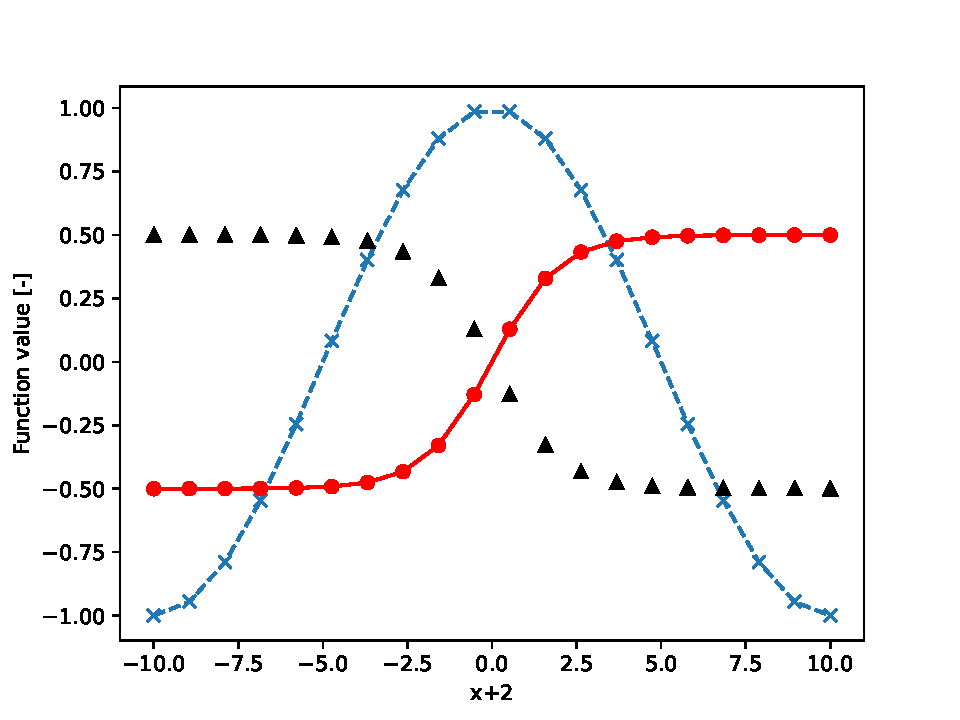
\includegraphics[width=\textwidth]{intro_matplotlib_3.pdf}
  \end{columns}
\end{frame}

{\nologo
\begin{frame}[fragile]
  \frametitle{Subplots}
  Multiple plots in a single figure are made by specifying a grid using \href{https://matplotlib.org/stable/api/_as_gen/matplotlib.pyplot.subplot.html#matplotlib-pyplot-subplot}{subplot}:
  \begin{columns}
    \column{0.5\textwidth}
    \begin{lstlisting}[language=Python]
x = np.linspace(0,2*np.pi,1000)
y1,y2 = np.sin(x), 2*np.cos(x)

# Specify figure size
fig = plt.figure(figsize=(8, 7))

# First index of 2x2 grid (top-left)
ax1 = plt.subplot(2, 2, 1) 
ax1.plot(x,y1)
ax1.set_title('sin(x)')

# Second index of 2x2 grid (top-right)
ax2 = plt.subplot(2, 2, 2) 
ax2.plot(x,y2)
ax2.set_title('cos(x)')

# Second index of 2x1 grid (whole bottom)
ax3 = plt.subplot(2, 1, 2) 
ax3.plot(x,y1**2+y2**2)
ax3.set_title(r'$\sin^2(x)+\cos^2(x)$')

plt.tight_layout()
plt.show()
    \end{lstlisting}\pause
    \column{0.5\textwidth}
      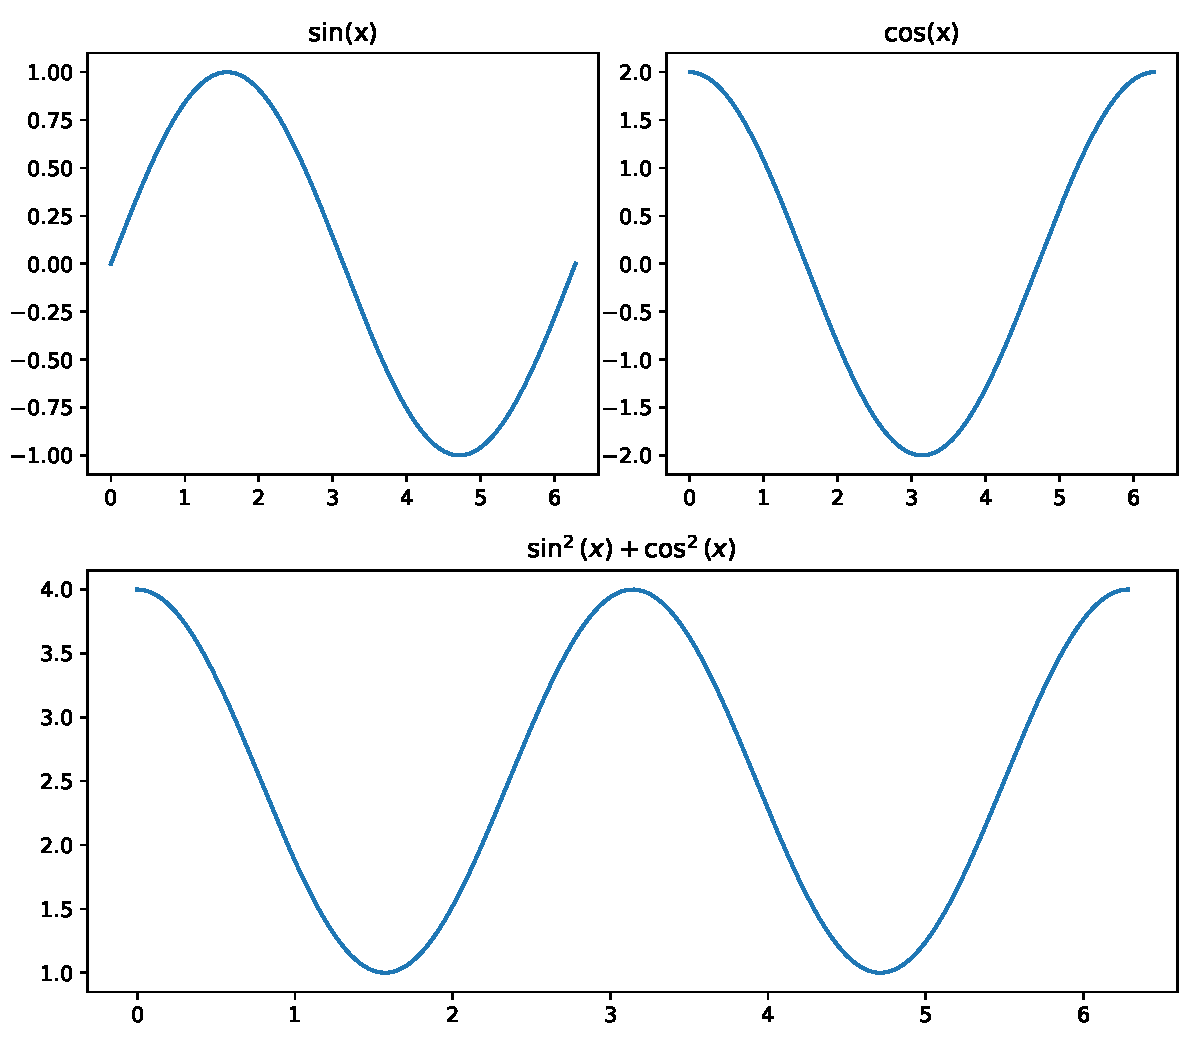
\includegraphics[width=\textwidth]{intro_matplotlib_4.pdf}
  \end{columns}
\end{frame}
}

% PRACTICE
\begin{frame}[fragile]
  \frametitle{Practice}
  Try to create the following figure:
  \begin{columns}
    \column{0.5\textwidth}
      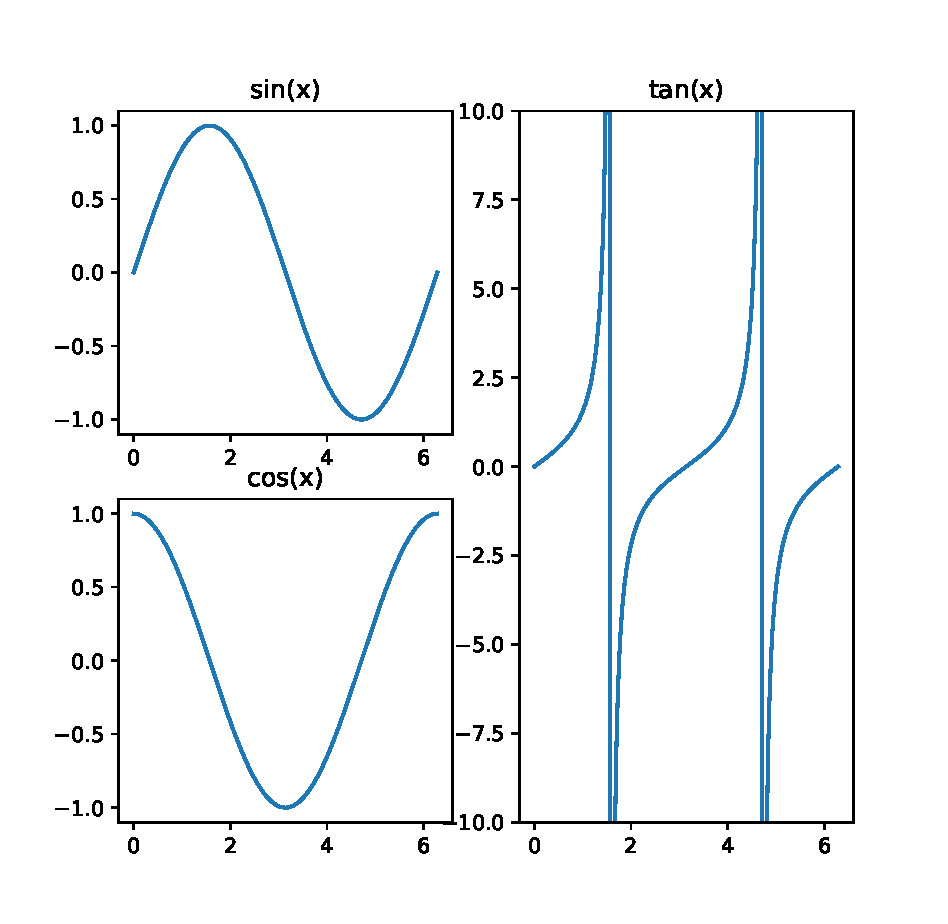
\includegraphics[width=\textwidth]{intro_matplotlib_5.pdf}

    \column{0.5\textwidth}
      % \begin{onlyenv}<beamer>
        \begin{lstlisting}[]
import numpy as np
import matplotlib.pyplot as plt
x = np.linspace(0,2*np.pi,1000)
y1,y2,y3 = np.sin(x), np.cos(x), np.tan(x)

ax1 = plt.subplot(2, 2, 1) 
ax1.plot(x,y1)
ax1.set_title('sin(x)')

ax2 = plt.subplot(2, 2, 3) 
ax2.plot(x,y2)
ax2.set_title('cos(x)')

# Second index of 2x1 grid (whole bottom)
ax3 = plt.subplot(1, 2, 2) 
ax3.plot(x,y3)
ax3.set_title('tan(x)')
ax3.set_ylim(-10, 10)
        \end{lstlisting}
      % \end{onlyenv}
  \end{columns}
\end{frame}

{\nologo
\subsection{Different plot styles}
\begin{frame}[fragile]
  \frametitle{2D plot styles}
  \begin{columns}[T]
    \column{0.4\textwidth}
      \begin{lstlisting}
import numpy as np
import matplotlib.pyplot as plt

x = np.linspace(-2*np.pi,2*np.pi,80)
y2 = 2*x**2 + 4*x - 3
y3 = 20*np.random.rand(y2.size)

ax1 = plt.subplot(2, 2, 1) 
ax1.plot(x,y2)
ax1.set_title('Line plot')

ax2 = plt.subplot(2, 2, 2) 
ax2.scatter(x,y3)
ax2.set_title('Scatter plot')

ax3 = plt.subplot(2, 2, 3) 
ax3.errorbar(x,y2,yerr=y3)
ax3.set_title('Errorbar')

ax4 = plt.subplot(2,2,4)
ax4.hist(y3)
ax4.set_title('Histogram')

plt.show()
      \end{lstlisting}
    \column{0.6\textwidth}
      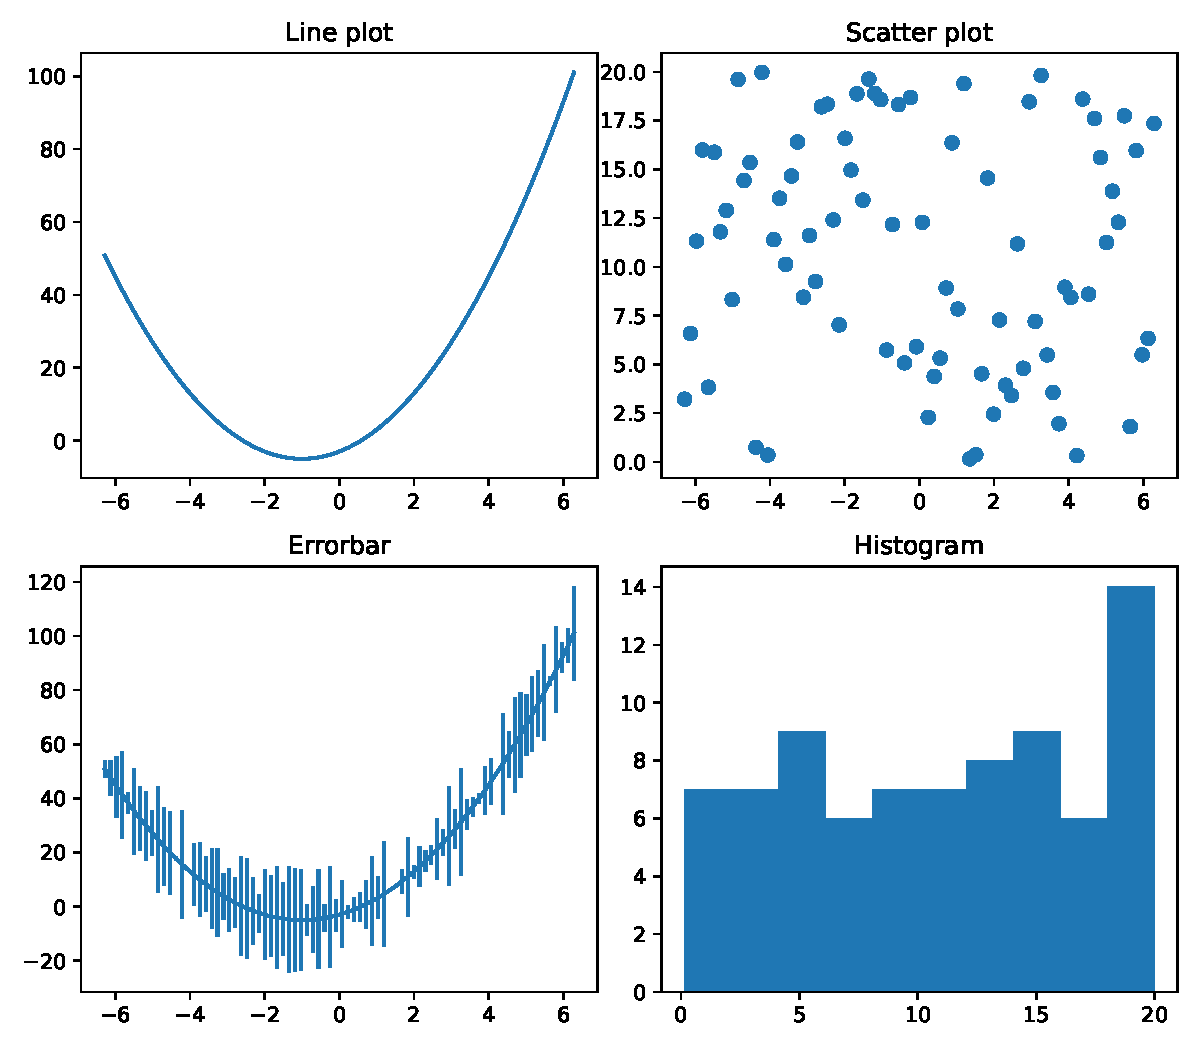
\includegraphics[width=\textwidth]{intro_matplotlib_6.pdf}
  \end{columns}
\end{frame}
}

\begin{frame}[fragile]
  \frametitle{Surface plot}
  We draw a surface plot of $\displaystyle f(x,y) = xy e^{\left(-x^2 -y^2 \right)}$:
  \begin{columns}
    \column{0.5\textwidth}
      \begin{lstlisting}[basicstyle=\tiny\ttfamily]
from mpl_toolkits.mplot3d import Axes3D
from matplotlib import cm
import matplotlib.pyplot as plt
import numpy as np

fig = plt.figure()
ax = fig.add_subplot(111, projection='3d')
(*@ \pause @*)
# Make data.
x = np.arange(-2, 2, 0.025)
y = np.arange(-2, 2, 0.025)
x,y = np.meshgrid(x, y)
z = x * y * np.exp(-x**2 - y**2)
(*@ \pause @*)
# Plot the surface.
surf = ax.plot_surface(x,y,z, 
        cmap=cm.magma,linewidth=0, antialiased=False)
(*@ \pause @*)
# Customize the z axis.
ax.set_zlim(-0.25, 0.25)

# Add a color bar which maps values to colors.
fig.colorbar(surf, shrink=0.5, aspect=5)

plt.show()
      \end{lstlisting}
    \column{0.5\textwidth}
      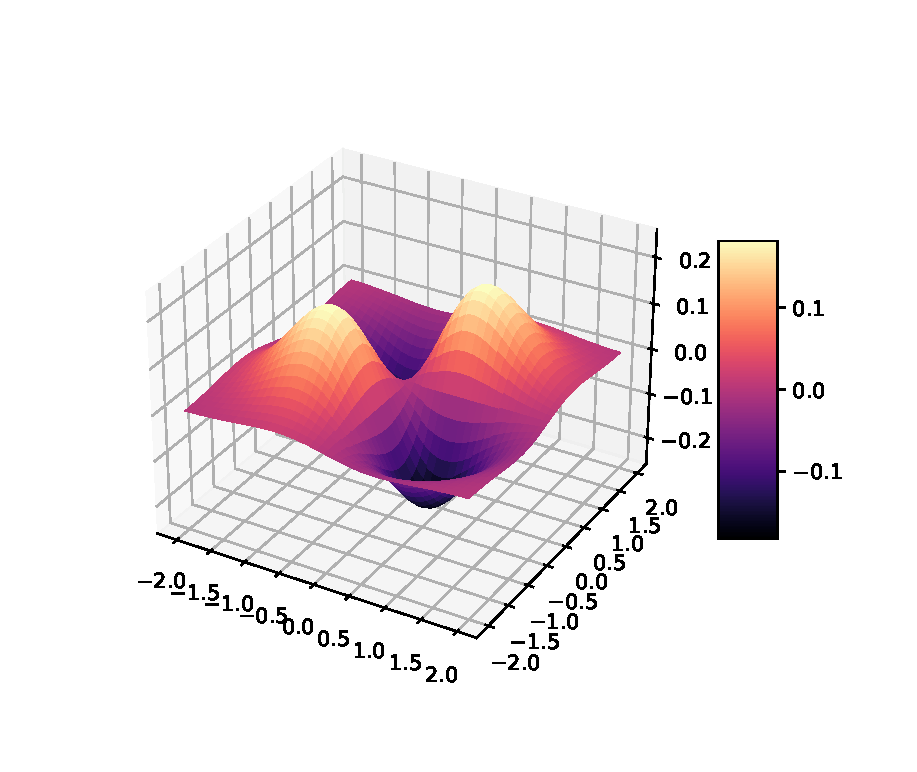
\includegraphics[width=\textwidth]{intro_matplotlib_7.pdf}
  \end{columns}
\end{frame}


\begin{frame}[fragile]
  \frametitle{Advanced plotting: Animating plots}
  The \lstinline|fig.canvas.draw()| and \lstinline|fig.canvas.flush_events()| methods hold the execution of your program until the graph is updated, facilitating a live view of the simulation result.
  \begin{lstlisting}
import numpy as np
import matplotlib.pyplot as plt

x = np.linspace(0, 4*np.pi, 100)
y = np.sin(x)

fig, ax = plt.subplots()
line, = ax.plot(x, y, '-')

ax.set_xlabel('X')
ax.set_ylabel('Y')
ax.set_title('Animating a Sine Wave')
plt.show(block=False)

for i in range(len(x)):
    line.set_data(x[:i+1], y[:i+1])
    fig.canvas.draw()
    fig.canvas.flush_events()
    plt.pause(0.01)
  \end{lstlisting}
\end{frame}


% \begin{frame}[fragile]
%   \frametitle{Other plotting tools}
%   \begin{columns}
%    \column{0.6\textwidth}
%     \begin{itemize}[<+->]
%       \item Error bars: \lstinline$plt.errorbar(x, y, yerr=err)$
%       \item 3D plots: \lstinline$ax.plot_trisurf(x, y, z)$
%       \item Histograms: \lstinline$plt.hist(x, bins=20)$
%     \end{itemize}
%    \column{0.4\textwidth}
%       \includegraphics<1>[width=\columnwidth]{show_errorbar-utc}
%       \mode<presentation>{
%         \includegraphics<2>[width=\columnwidth]{show_ezplot3-utc}
%         \includegraphics<3>[width=\columnwidth]{show_hist-utc}
%     }
%  \end{columns}
% \end{frame}

% \subsection*{Multi-dimensional data}
% \begin{frame}<handout:3>[fragile]
%   \frametitle{Multi-dimensional data}
%   Python typically requires the definition of rectangular grid coordinates using \lstinline$np.meshgrid$:\\
%   \begin{overlayarea}{\textwidth}{6cm}
%   \begin{columns}[T]
%    \column{0.6\textwidth}
%     \begin{lstlisting}[language=Python]
% x, y = np.meshgrid(np.linspace(-2, 2, 41), np.linspace(-2, 2, 41))
% z = x * y * np.exp(-x**2 - y**2)
%     \end{lstlisting}
%     \vskip1em
%     \begin{itemize}
%       \item<2-> Surface plot
%       \item<3-> Contour plot
%       \item<4-> Waterfall 
%       \item<5> Ribbons
%     \end{itemize}
%    \column{0.4\textwidth}
%    \begin{center}
%       \includegraphics<2>[width=\columnwidth]{show_surf}
%       \mode<presentation>{
%         \includegraphics<3>[width=\columnwidth]{show_contour}
%         \includegraphics<4>[width=\columnwidth]{show_waterfall}
%         \includegraphics<5>[width=\columnwidth]{show_ribbon}
%       }
%    \end{center}
%     \only<2>{
%       \lstinline$ax.plot_surface(x, y, z)$
%     }
%     \mode<presentation>{
%       \only<3>{
%         \lstinline$v = np.linspace(-0.5, 0.5, 21)$\\
%         \lstinline$cs = ax.contour(x, y, z, levels=v)$\\
%         \lstinline$ax.clabel(cs, inline=1, fontsize=10)$
%       }
%       \only<4>{
%       \lstinline$ax.plot_trisurf(x.flatten(), y.flatten(), z.flatten(), cmap='winter')$
%       }
%       \only<5>{
%       \lstinline$ax.plot_trisurf(x.flatten(), y.flatten(), z.flatten(), cmap='viridis', linewidth=0, antialiased=False)$
%       }
%     }
%  \end{columns}
%  \end{overlayarea}
% \end{frame}

% \begin{frame}[fragile]
%   \frametitle{Vector data}
%   The gradient function, as expected, is used to obtain the gradient of a scalar field. Colors can be used in the background to simultaneously plot field data:
%   \begin{columns}[T]
%    \column{0.6\textwidth}
%     \begin{lstlisting}[language=Python]
% x, y = np.meshgrid(np.linspace(-2, 2, 21), np.linspace(-2, 2, 21))
% z = x * y * np.exp(-x**2 - y**2)
% dx, dy = np.gradient(z, 0.4, 0.4)

% # Background
% cs = plt.contourf(x, y, z, 30, cmap='hot')
% plt.colorbar(cs)

% plt.axis('tight')

% # Vectors
% plt.quiver(x, y, dx, dy, color='k')
%     \end{lstlisting}
%    \column{0.4\textwidth}
%    \begin{center}
%       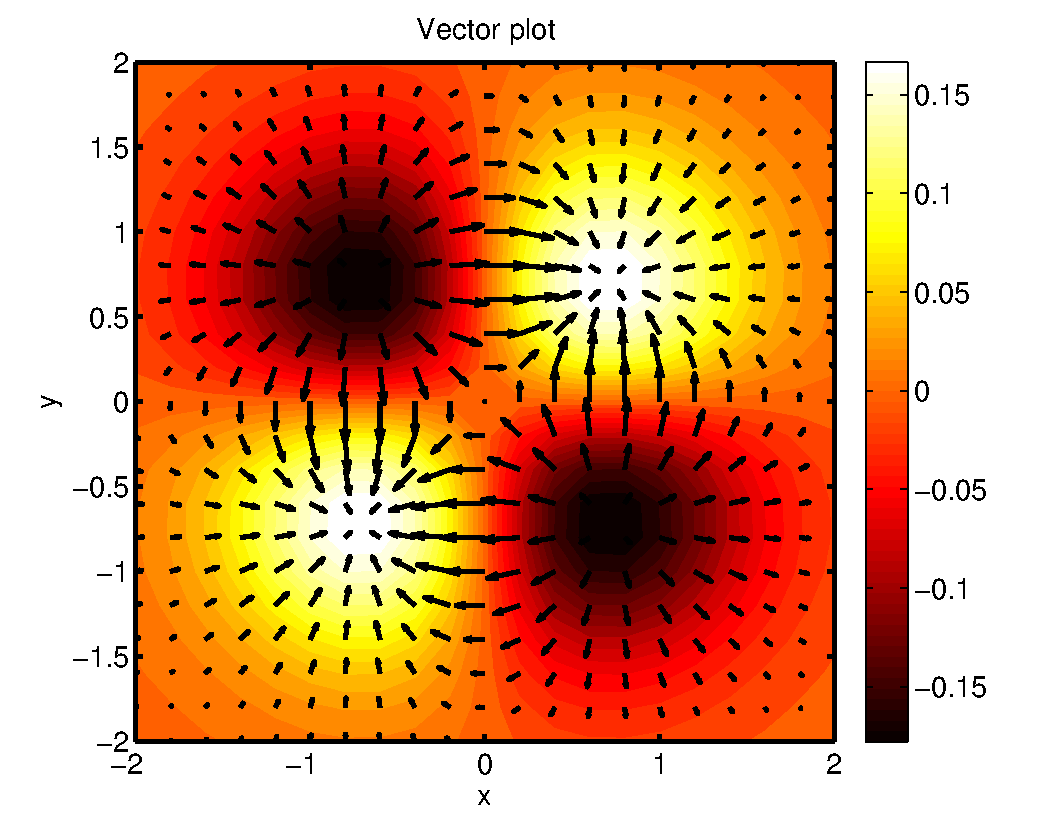
\includegraphics[width=\columnwidth]{show_vector}
%     \end{center}
%   \end{columns}
% \end{frame}

% \begin{frame}[fragile]
%   \frametitle{Enhancing Plots in Matplotlib (2)}
%   \begin{columns}
%     \column{0.4\textwidth}
%   Matplotlib offers various ways to enhance your plots, including adding labels, titles, and grids.\pause
%   \begin{lstlisting}[language=Python]
% plt.plot(x, y, 'r-o')
% plt.xlabel('X-axis label')
% plt.ylabel('Y-axis label')
% plt.title('Plot Title')
% plt.grid(True)
% plt.show()
%   \end{lstlisting}\pause
%    \column{0.5\textwidth}
%    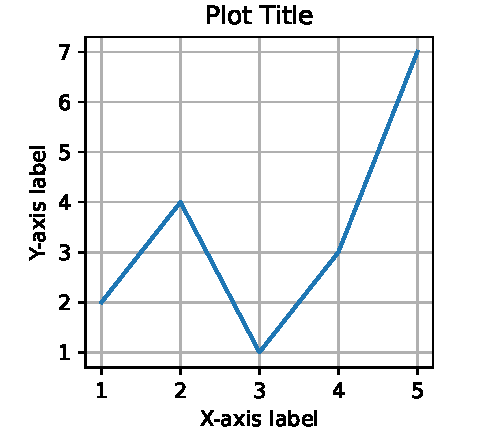
\includegraphics[width=0.6\textwidth]{intro_matplotlib2.pdf}
%   \end{columns}

%   \begin{columns}
%     \column{0.4\textwidth}
%   Creating scatter and bar plots:
%   \begin{lstlisting}[language=Python]
% plt.scatter(x, y, color='red')
% plt.show
% plt.bar(x, y, color='green')
% plt.show()
%   \end{lstlisting}
%   \column{0.5\textwidth}
%   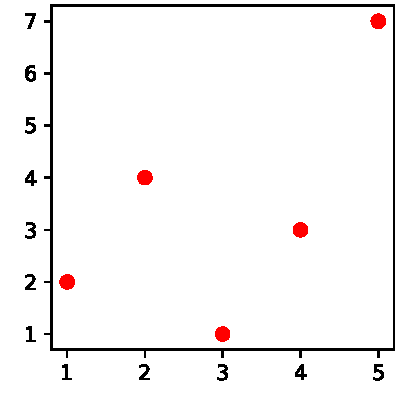
\includegraphics[width=0.4\textwidth]{intro_matplotlib3.pdf}
%   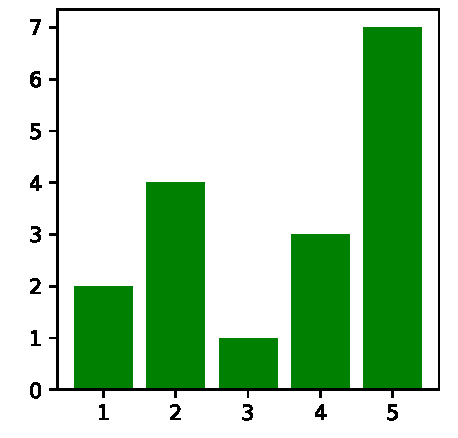
\includegraphics[width=0.4\textwidth]{intro_matplotlib4.pdf}
%   \end{columns}
% \end{frame}

% \begin{frame}
%   \frametitle{Some of the plots of Matplotlib}
%   \begin{figure}
%     \centering
%     \begin{minipage}{.25\textwidth}
%       \centering
%       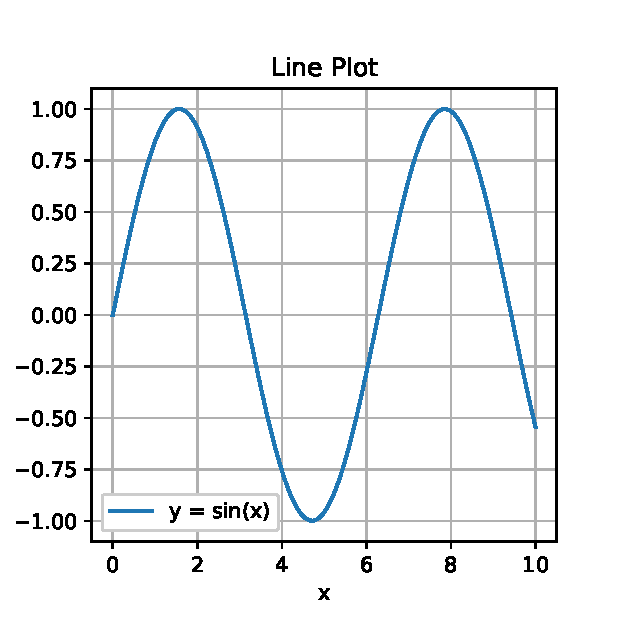
\includegraphics[width=0.99\linewidth]{mpl_plot_examples/line_plot.eps} %FILL IN THE PIC PATH HERE for plot
%     \end{minipage}%
%     \begin{minipage}{.25\textwidth}
%       \centering
%       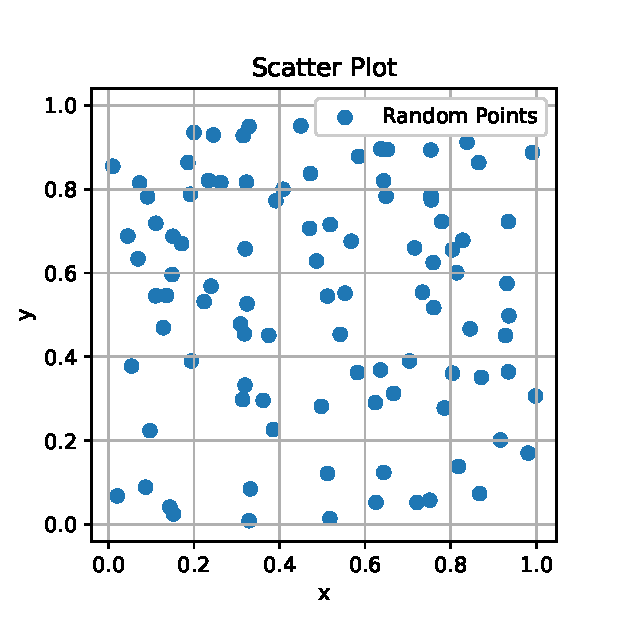
\includegraphics[width=.99\linewidth]{mpl_plot_examples/scatter_plot.eps} %FILL IN THE PIC PATH HERE for scatter
%     \end{minipage}
%   \end{figure}

%   \begin{figure}
%     \centering
%     \begin{minipage}{.25\textwidth}
%       \centering
%       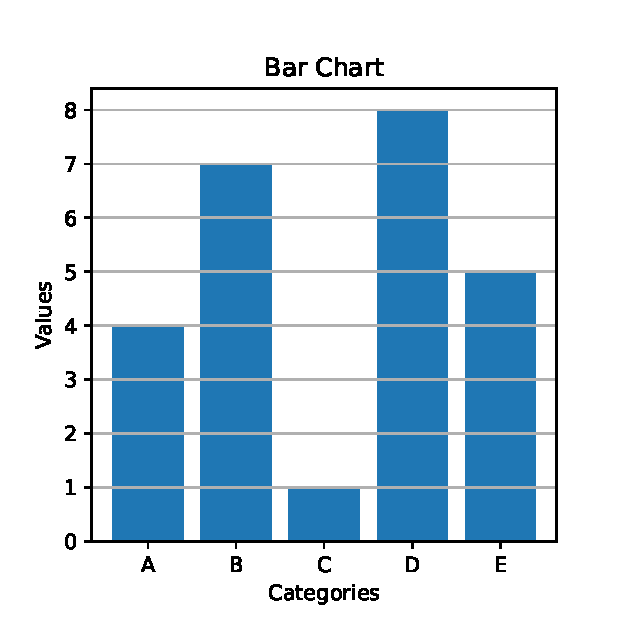
\includegraphics[width=.99\linewidth]{mpl_plot_examples/bar_chart.eps} %FILL IN THE PIC PATH HERE for bar
%     \end{minipage}%
%     \begin{minipage}{.25\textwidth}
%       \centering
%       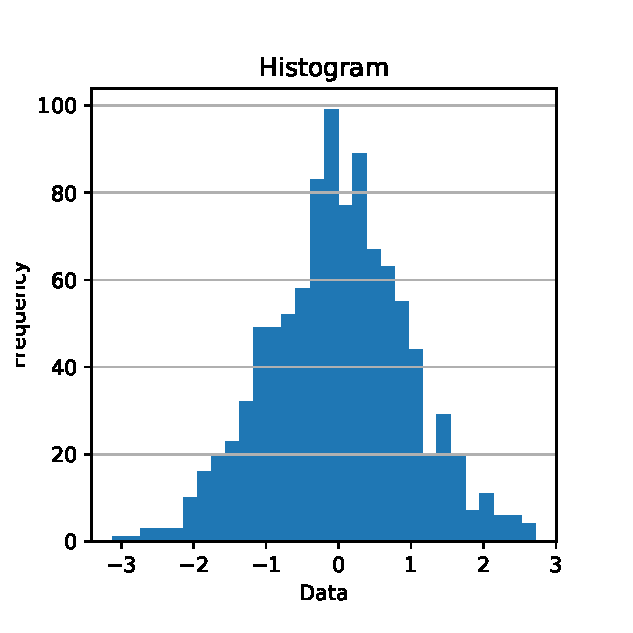
\includegraphics[width=.99\linewidth]{mpl_plot_examples/histogram.eps} %FILL IN THE PIC PATH HERE for hist
%     \end{minipage}
%     \begin{minipage}{.25\textwidth}
%       \centering
%       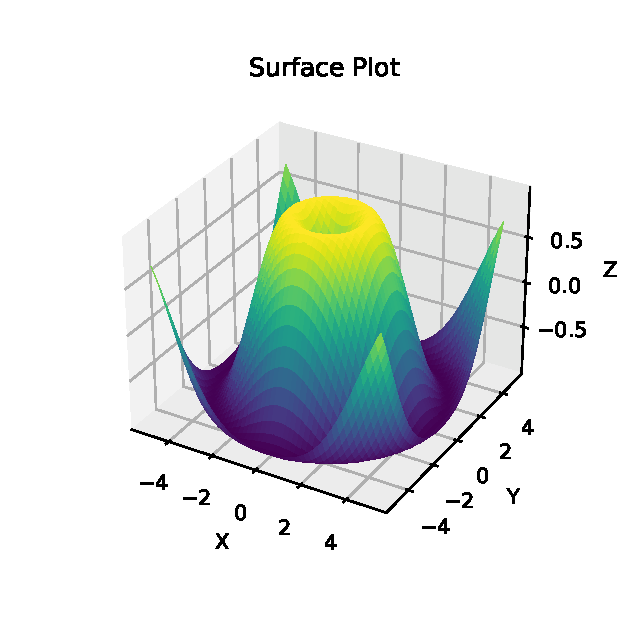
\includegraphics[width=.99\linewidth]{mpl_plot_examples/surface_plot.eps} %FILL IN THE PIC PATH HERE for surface
%     \end{minipage}
%   \end{figure}
% \end{frame}




% INPUT AND OUTPUT
\section{IO}
\subsection{Input/output}
\againframe<2>{contents_prog2}

\begin{frame}[fragile]
  \frametitle{Input and Output in Python (1)}
  Many programs require some input (data) to function correctly. A combination of the following is common:
  \begin{itemize}[<+->]
    \item Input may be given in a parameters file (``hard-coded'')
    \item Input may be entered via the keyboard using the `input` function:
    \begin{lstlisting}[language=Python,numbers=none]
>>> a = input('Please enter a number: ')
    \end{lstlisting}
    \item Input may be read from a file, for instance using Python's built-in open function or libraries like `numpy` for more complex data structures:
    \begin{lstlisting}[language=Python,numbers=none]
>>> with open('myData.txt', 'r') as file:
>>>     data = file.read()
>>> 
>>> import numpy as np
>>> data = np.loadtxt("my_file.csv")
    \end{lstlisting}
    \item There are many other libraries and functions for more advanced input operations, such as json, xml, etc.
  \end{itemize}
 \end{frame}

 \begin{frame}[fragile]
  \frametitle{Input and Output in Python (2)}
  Output of results can be done in several ways, including:
  \begin{itemize}[<+->]
    \item Displaying results to the console - simply omitting a print statement will automatically show expression results in most Python IDEs.
    \item Using the `print` function to show results in the console:
    \begin{lstlisting}[language=Python,numbers=none]
>>> print("The result is:", result)
    \end{lstlisting}
    \item Saving data to a file can be done using various methods including writing to a file or using libraries like pandas for structured data:
    \begin{lstlisting}[language=Python,numbers=none]
>>> with open('output.txt', 'w') as file:
>>> file.write(str(data))

>>> data.save("data.npy")
    \end{lstlisting}
    \item More advanced output methods can utilize libraries such as NumPy, pandas, etc. to save data in various formats including JSON, Excel, etc.
  \end{itemize}
 \end{frame}



\section{Coding style}
\subsection{Program design}
\againframe<2>{contents_prog2}

\begin{frame}[label=workrightfast]
  \frametitle{Make a habit of the following adage}
  \begin{center}
    
\includegraphics[width=0.8\textwidth]{workrightfast.pdf}
  \end{center}
\end{frame}

{\nologo
\begin{frame}[label=work-explain]
  \frametitle{Make it work}
  Use the building blocks of previous lecture to create an algorithm:
  \begin{enumerate}
    \colorize<1> \item \emph{Problem analysis}\\ Contextual understanding of the nature of the problem to be solved
    \colorize<2> \item \emph{Problem statement}\\ Develop a detailed statement of the mathematical problem to be solved with the program
    \colorize<3> \item \emph{Processing scheme}\\ Define the inputs and outputs of the program
    \colorize<4> \item \emph{Algorithm}\\ A step-by-step procedure of all actions to be taken by the program (\emph{pseudo-code})
    \colorize<5> \item \emph{Program the algorithm}\\ Convert the algorithm into a computer language, and debug until it runs
    \colorize<6> \item \emph{Evaluation}\\ Test all of the options and conduct a validation study
  \end{enumerate}
  \vskip1em
  Now it's time to make it right!
\end{frame}
}
% \subsection*{Program design and coding style}
% \begin{frame}
%   \frametitle{It's a bit disturbing but...}
%   \begin{center}
%     {\LARGE Your code will not be understood by anyone\\}
%   \pause
%   \vskip1em
%   That includes future-you
%   \vskip2em
%   \end{center}
% \end{frame}

\subsection*{Example code}
\begin{frame}[fragile]
 \frametitle{Interpret the following code}
 \begin{lstlisting}
s = checksc()
if s:
    a = cb()
    b = cfrsp()
    if a < 5:
        if b > 5:
            a = gtbs()
        if a > b:
            ubx()
else:
    brn()
    gtbs()
 \end{lstlisting}
\end{frame}

\begin{frame}[plain]

\includegraphics[keepaspectratio=true,width=\textwidth]{wat-2.jpg}
\end{frame}

\begin{frame}[fragile]
 \frametitle{Enhancing Readability with Proper Indentation}
 Proper indentation is not just about syntax in Python; it significantly impacts the readability of the code. Python recommends 4 spaces for indentation. Let's see the difference:
 \pause
 \begin{columns}[T]
    \column{0.5\textwidth}
     \begin{lstlisting}
s = checksc()
if s:
a = cb()
b = cfrsp()
if a < 5:
if b > 5:
a = gtbs()
if a > b:
ubx()
else:
brn()
gtbs()
 \end{lstlisting}
    \column{0.5\textwidth}
     \begin{lstlisting}
s = checksc()
if s:
    a = cb()
    b = cfrsp()
    if a < 5:
        if b > 5:
            a = gtbs()
        if a > b:
            ubx()
else:
    brn()
    gtbs()
 \end{lstlisting}
 \end{columns}
\end{frame}

\begin{frame}[fragile]
 \frametitle{Readable Variables and Function Names}
 Making use of descriptive variable and function names enhances the readability and understanding of the code. 
 \begin{columns}[T]
    \column{0.5\textwidth}
\begin{lstlisting}
s = checksc()
if s:
    a = cb()
    b = cfrsp()
    if a < 5:
        if b > 5:
            a = gtbs()
        if a > b:
            ubx()
else:
    brn()
    gtbs()
 \end{lstlisting}
    \column{0.5\textwidth}
     \begin{lstlisting}
isAvailable = checkSchedule()
if isAvailable:
    bookCount = countBooks()
    freeShelfSpace = checkFreeShelfSpace()
    if bookCount < 5:
        if freeShelfSpace > 5:
            bookCount = visitBookStore()
        if bookCount > freeShelfSpace:
            useStorageBox()
else:
    burnBooks()
    visitBookStore()
 \end{lstlisting}
 \end{columns}
\end{frame}

\begin{frame}[fragile]
 \frametitle{Avoiding Magic Numbers in the Code}
 Magic numbers are constant values without a name, which can reduce code readability. Replacing them with named constants can enhance the understanding of the code.
 \begin{columns}[T]
    \column{0.5\textwidth}
     \begin{lstlisting}
isAvailable = checkSchedule()
if isAvailable:
    bookCount = countBooks()
    freeShelfSpace = checkFreeShelfSpace()
    if bookCount < 5:
        if freeShelfSpace > 5:
            bookCount = visitBookStore()
        if bookCount > freeShelfSpace:
            useStorageBox()
else:
    burnBooks()
    visitBookStore()
 \end{lstlisting}
    \column{0.5\textwidth}
     \begin{lstlisting}[language=Python,emph={MIN_BOOKS_REQUIRED,MAX_SHELF_SPACE},emphstyle=\color{red}]
MAX_SHELF_SPACE = 5
MIN_BOOKS_REQUIRED = 5

isAvailable = checkSchedule()
if isAvailable:
    bookCount = countBooks()
    freeShelfSpace = checkFreeShelfSpace()
    if bookCount < MAX_SHELF_SPACE:
        if freeShelfSpace > MIN_BOOKS_REQUIRED:
            bookCount = visitBookStore()
        if bookCount > freeShelfSpace:
            useStorageBox()
else:
    burnBooks()
    visitBookStore()
 \end{lstlisting}
 \end{columns}
\end{frame}

\begin{frame}[fragile]
 \frametitle{Now, That's More Like It!}
 Demonstrating the evolution of the script to a more readable and maintainable version.
 \begin{columns}[T]
    \column{0.3\textwidth}
     \begin{lstlisting}[language=Python]
s = checksc()
if s:
    a = cb()
    b = cfrsp()
    if a < 5:
        if b > 5:
            a = gtbs()
        if a > b:
            ubx()
else:
    brn()
    gtbs()
 \end{lstlisting}
    \column{0.7\textwidth}
     \begin{lstlisting}[language=Python]
MAX_SHELF_SPACE = 5
MIN_BOOKS_REQUIRED = 5

isAvailable = checkSchedule()
if isAvailable:
    bookCount = countBooks()
    freeShelfSpace = checkFreeShelfSpace()
    if bookCount < MAX_SHELF_SPACE:
        if freeShelfSpace > MIN_BOOKS_REQUIRED:
            bookCount = visitBookStore()
        if bookCount > freeShelfSpace:
            useStorageBox()
else:
    burnBooks()
    visitBookStore()
 \end{lstlisting}
 \end{columns}
\end{frame}


%% ASPECTS OF A GOOD PROGRAM
\subsection*{Aspects of a good program}
\begin{frame}
  \frametitle{Writing readable code}
  Good code reads like a book.\vskip2em \pause
  \begin{itemize}
    \item When it doesn't, make sure to use comments. In Python, everything following \lstinline$ \# is a comment$
    \item Prevent ``smart constructions'' in the code
    \item Re-use working code (i.e. create functions for well-defined tasks).
    \item Documentation is also useful, but hard to maintain.
    \item Python comes with a function that generates reports from comments
  \end{itemize}
\end{frame}

\begin{frame}[fragile]
  \frametitle{How not to comment}
  \begin{itemize}[<+->]
   \item Useless:
   \begin{lstlisting}
# Start program 
   \end{lstlisting}
   \item Obvious:
   \begin{lstlisting}
if (a > 5)   # Check if a is greater than 5
    ... 
 \end{lstlisting}
   \item Too much about the life:
   \begin{lstlisting}[basicstyle=\tiny\ttfamily]
# Well... I do not know how to explain what is going on
# in the snippet below. I tried to code in the night 
# with some booze and it worked then, but now I have a 
# strong hangover and some parameters still need to be
# worked out...
   \end{lstlisting}
 
   \item ...
   \begin{lstlisting}[basicstyle=\tiny\ttfamily]
# You may think that this function is obsolete, and doesn't seem to
# do anything. And you would be correct. But when we remove this 
# function for some reason the whole program crashes and we can't 
# figure out why, so here it will stay.
   \end{lstlisting}
  \end{itemize}
 \end{frame}
 
 \begin{frame}[fragile]
  \frametitle{Adding comments to our Python program}
  \centering\tikz{\node[emphblock, text width=0.7\textwidth]{Use comments to document design and purpose (functionality), not mechanics (implementation).};}
  \begin{lstlisting}
IAmFree = checkSchedule()
if IAmFree:
    # Count books and amount of free space on a shelf. 
    # If minimum number of books I need is less than a 
    # shelf capacity, go shopping and buy additional 
    # literature. If the amount of books after the 
    # shopping is too big, use boxes to store them.
    books = countBooks()
    shelfSize = countFreeSpaceShelf()
    
    ...
    
else:
    burnBooks()
    goToBookStore()
 \end{lstlisting}
 \end{frame}

\begin{frame}
  \frametitle{What else makes a good program?}
  \begin{columns}[T]
        \column{0.5\textwidth}
        \begin{itemize}
            \item Portability (guaranteed in Python)
            \item Readability
            \item Efficiency 
            \item Structural
            \item Flexibility
            \item Generality
            \item Documentation
        \end{itemize}
        \column{0.5\textwidth}
Funny thing is: This list does not mention that the program should be actually working for its intended purposes!
    \end{columns}
\end{frame}

\begin{frame}[fragile]
  \frametitle{Readability}
  Don't use meaningless variable or function names. Rule of thumb: use verbs for functions and nouns for variables.
  \vspace*{2em}
  \begin{lstlisting}[language=Python]
# stupid names
x = 5;
xx = myfunction(x);

# proper names
number_dams = 6;
beaver_workforce = allocate_beavers();
dams = build_dams(beaver_workforce, number_dams);
  \end{lstlisting}
\end{frame}

\begin{frame}[fragile]
  \frametitle{Efficiency}
  This one is difficult. Not much you can do without truly understanding how Python is utilizing your processor and memory. A couple of guidelines though:
  \begin{itemize}
      \item Avoid loops
      \item Especially avoid nested loops
      \item Use inherent matrix operations when possible
      \item Reduce IO (i.e. reading / writing to and from files)
      \item Don't run scripts from network disks
      \item Pre-allocate your arrays, that means, making it as large as the maximum required size for your particular problem
      \item Use Python's built-in modules for performance profiling, such as cProfile or timeit, to test the execution times
  \end{itemize}
\end{frame}

\begin{frame}[fragile]
  \frametitle{Efficiency: Measuring execution time example}
  \begin{columns}
    \column{0.5\textwidth}
    \begin{lstlisting}[language=Python]
import numpy as np
import time

x = np.linspace(0, 10, 1000001)
start_time = time.time()

y = []
for cr in range(len(x)):
    y.append(np.sin(2 * np.pi * x[cr]))

end_time = time.time()
print(f'Execution time: {end_time - start_time} seconds')
    \end{lstlisting}
    \column{0.5\textwidth}
    \begin{lstlisting}[language=Python]
import numpy as np
import time

x = np.linspace(0, 10, 1000001)
start_time = time.time()

y = np.sin(2 * np.pi * x)

end_time = time.time()
print(f'Execution time: {end_time - start_time} seconds')
    \end{lstlisting}
  \end{columns}
\end{frame}

\begin{frame}[fragile]
  \frametitle{Structural}
  \begin{itemize}
      \item Compartmentalize your code.
      \item Write functions whenever possible.
      \begin{itemize}
        \item If you have $>15$ lines of code, you can probably replace it by one or more functions.
        \item In principle, it should not even matter how function works, as long as it gives the expected output.\\ \vskip1ex
        \begin{tikzpicture}[node distance = 3cm, auto]
          % Place nodes
          \node [emphblock] (function) {Function};
          \node [emphblock, left of=function] (input) {Input};
          \node [emphblock, right of=function] (output) {Output};
          % Draw edges
          \draw [line,->] (input) -> (function);
          \draw [line,->] (function) -> (output);
      \end{tikzpicture}\vskip1ex
      \end{itemize}
      \item Put critical variables at the beginning of your program.
  \end{itemize}  
\end{frame}

\begin{frame}[fragile]
  \frametitle{Structural}
    Write code as though it were paragraphs in a story.
    \begin{lstlisting}[language=Python]
from dependencies import * # importing all dependencies

# Step 0: Define variables
n_steps = 10000  # number of steps
n_walks = 1000  # number of random walk samples

# Step 1: Generate n_walks number of random walks
de = np.zeros((n_walks, 2))
for i in range(n_walks):
    angles = get_random_angles(n_steps)
    coord = transform_angles_to_coordinates(angles)
    de[i, 0] = calculate_de(coord)  # store de
    de[i, 1] = de[i, 0]**2  # store de^2

# Step 2: Plot the histogram
plt.hist(de[:, 0], density=True)
D, P = calculate_pdf(n_steps, 1000)
plt.plot(D, P)
plt.show()
    \end{lstlisting}
\end{frame}


\begin{frame}[fragile]
  \frametitle{Flexibility}
    If you want to add a feature or change something inside the program, it should not require rewriting the whole program. (jargon: non-linear propagation of change).\\
    
    Solution: Encapsulate your code and "Don't Repeat Yourself"
    \begin{itemize}
        \item Use functions for specific tasks (can you verbalize it? Then it is probably a function)
        \item Use variables, even for constants (it sounds like a oxymoron, but it's not! In fact, constant variables are a real thing)
        \item Use abstraction whenever possible
    \end{itemize}
\end{frame}

\begin{frame}[fragile]
  \frametitle{Generalization}
    If your code works for one problem, it should also work for a similar problem, whether it's in another company or on another planet. \\ \vskip1em
    
    Pro-tip: Separate data from algorithms.\\
    
    To be honest, I rarely see students making this mistake.
    
\begin{lstlisting}
# Stupid code
A = [[1, 2, 3], [4, 5, 6], [7, 8, 9]]  # Hardcode data in the program
    
# Smart code
with open('some_random_dataset.dat') as file:
    data = file.read()  # or use appropriate data loading functions from libraries like pandas
\end{lstlisting}
\end{frame}


\begin{frame}[fragile]
  \frametitle{Documentation}
    Properly document your code. Write your comments in a clear and concise fashion. Help your future self: Write clear and concise documentation.
    \begin{columns}
    \column{0.6\textwidth}
    \begin{lstlisting}[language=Python]
def f(a, b=None):
    if b is not None:
        c = a + b
    elif b is None and a is not None:
        c = a + a
    else:
        c = 0
    return c
    \end{lstlisting}
    \column{0.4\textwidth}
    
\includegraphics[width=\columnwidth]{figures/drakeno.jpg}
    \end{columns}
\end{frame}

\begin{frame}[fragile]
  \frametitle{Documentation}
    Properly document your code. Write your comments in a clear and concise fashion. Help your future self: Write clear and concise documentation.
    \begin{columns}
    \column{0.6\textwidth}
    \begin{lstlisting}[language=Python]
def f(a, b=None):
    """
    Add two values together.
    
    Parameters:
    a: The first number.
    b: The second number. Optional.
    
    Returns:
    The sum of a and b, or 2*a if b is not given, or 0 if a is not given.
    
    See also: sum, operator.add
    """
    if b is not None:
        c = a + b  # sum two different numbers
    elif b is None and a is not None:
        c = a + a  # double single number
    else:
        c = 0      # input not valid
    return c
    \end{lstlisting}
    \column{0.4\textwidth}
    
\includegraphics[width=\columnwidth]{figures/drakeyes.jpg}
    \end{columns}
\end{frame}


\againframe{workrightfast}

\begin{frame}[fragile,label=wrf-explain]
  \frametitle{Make a habit of the following adage}
  \begin{enumerate}
    \colorize<1> \item \emph{Make it work}\\ 
    Create an algorithm that does the intended job. Make sure it works, and works repeatedly. Test and verify frequently. Add \emph{todo} comments when you're not sure about a certain decision.
    \colorize<2> \item \emph{Make it right}\\ 
    Refactor the code to improve the code design. Insert functions, comments, compartmentalize it. Get rid of magic numbers, use sensible variable names. Check input. Test and verify. Align with the team!
    \colorize<3> \item \emph{Make it fast}\\ 
    Measure and tune the performance of your code (profiling tool). In Python, vectorized calculations are much (!) faster than for-loops. Use sensible numerical techniques (e.g. higher-order integration).
  \end{enumerate}
  Program by iterating over these aspects multiple times, starting at the fine-grained level, working your way up.
\end{frame}

% \begin{frame}
% \frametitle{Code organization}
%   \begin{itemize}
%     \item Optimization of a code is time-consuming and complicated
%     \item The more you optimize your code, the less readable it becomes
%     \item But... You can write it in a such way that it will be flexible and easy to maintain
%     \item Especially important in team work
%     \item Any person has its own handwriting. Any programmer has its own coding style.
% \end{itemize}
%  \tikz{\node[emphblock,text width=\textwidth]{The coding style $\equiv$ handwriting...};}
% \end{frame}

\section{Debugging and profiling}
\subsection*{Errors in programming}
\againframe<2>{contents_prog2}
\begin{frame}
 \frametitle{Errors in computer programs}
 \footnotesize\selectfont
 The following symptoms can be distinguished:
 \begin{itemize}
   \item Unable to execute the program
   \item Program crashes, warnings or error messages
   \item Never-ending loops
   \item Wrong (unexpected) result
 \end{itemize}
 \vskip1em
 \uncover<2->{
  Three error categories:
  \begin{description}
   \colorize<2->  \item[Syntax errors] You did not obey the language rules. These errors prevent running or compilation of the program.
   \colorize<3->  \item[Runtime errors] Something goes wrong during the execution of the program resulting in an error message (problem with input, division by zero, loading of non-existent files, memory problems, etc.)
   \colorize<4->  \item[Semantic errors] The program does not do what you expect, but does what have told it to do.
  \end{description}
 }
\end{frame}

% \begin{frame}[fragile]
%  \frametitle{Verification and validation}
%   \scriptsize\selectfont
%   \begin{columns}
%     \column{0.6\textwidth}
%     \uncover<3->{\begin{block}{Verification}
%     Verification is the process of mathematically and computationally assuring that the model computes what you have entered.    
%     \end{block}
%     }
%     \uncover<7->{
%     \begin{block}{Validation}
%       Validation is the process of determining the degree to which a model is an accurate representation of the real world from the perspective of the intended uses of the model
%     \end{block}
%     }
% 
%   \column{0.4\textwidth}
%     \begin{tikzpicture}[block/.style={rectangle,minimum size=3mm,text badly centered,drop shadow,
% 					thick,rounded corners,draw=maincolor,top color=maincolor!35,bottom color=maincolor!20,
% 					font=\sffamily\scriptsize},>=stealth,node distance=0.75cm]
% 	\node[block] (p) at (0,0) {Problem};
% 	\uncover<2->{\node[below of=p] (p1) {};
% 	\node[block, below of=p1] (mm) {Mathematical Model};
% 	\node[below of=mm] (mm1) {};}
% 	\uncover<4->{\node[block, below of=mm1] (cm) {Computational Model};
% 	\node[below of=cm] (cm1) {};}
% 	\uncover<6->{\node[block, below of=cm1] (r) {Results};}
% 	
% 	\uncover<3->{\node[block, left of=p1,node distance=2cm] (v1) {Verification};}
% 	\uncover<5->{\node[block, left of=mm1,node distance=2cm] (v2) {Verification};}
% 	\uncover<7->{\node[block, left of=cm1,node distance=2cm] (v3) {Validation};}
% 	
% 	\uncover<2->{\draw[->] (p) -> (mm);}
% 	\uncover<4->{\draw[->] (mm) -> (cm);}
% 	\uncover<6->{\draw[->] (cm) -> (r);}
% 	
% 	\uncover<3->{\draw[->] (v1) -> (p1);}
% 	\uncover<5->{\draw[->] (v2) -> (mm1);}
% 	\uncover<7->{\draw[->] (v3) -> (cm1);}
%     \end{tikzpicture}
%   \end{columns}
% 
% \end{frame}
% % 
% 
% \begin{frame}
%   \frametitle{Be aware of your uncertainties}
%   \scriptsize\selectfont
%   \begin{columns}
%     \column{0.5\textwidth}
%     \begin{center}
%       \mode<beamer>{
% 	\includegraphics<1>[width=0.8\columnwidth]{ptolemy1-1}
% 	\includegraphics<2>[width=0.8\columnwidth]{ptolemy1-2}
% 	\includegraphics<3>[width=0.8\columnwidth]{ptolemy1-3}
% 	\includegraphics<4>[width=0.8\columnwidth]{ptolemy1-4}
% 	\includegraphics<5>[width=0.8\columnwidth]{ptolemy1-5}
% 	\includegraphics<6>[width=0.8\columnwidth]{ptolemy1-6}
%       }
%       \includegraphics<7->[width=0.8\columnwidth]{ptolemy1-7}
%     \end{center}
%     \column{0.5\textwidth}
%     \begin{center}
%       \mode<beamer>{
% 	\includegraphics<7>[width=0.8\columnwidth]{ptolemy2-0}
% 	\includegraphics<8>[width=0.8\columnwidth]{ptolemy2-1}
% 	\includegraphics<9>[width=0.8\columnwidth]{ptolemy2-2}
% 	\includegraphics<10>[width=0.8\columnwidth]{ptolemy2-3}
% 	\includegraphics<11>[width=0.8\columnwidth]{ptolemy2-4}
% 	\includegraphics<12>[width=0.8\columnwidth]{ptolemy2-5}
% 	\includegraphics<13>[width=0.8\columnwidth]{ptolemy2-6}
%       }
%       \includegraphics<14>[width=0.8\columnwidth]{ptolemy2-7}
%     \end{center}
%   \end{columns}
%   \begin{itemize}
%     \item<7-> The perceived orbit of Mars from Earth shows a zig-zag (in contrast to the Sun, Mercury, Venus)
%     \item<14> Even though they were not 'right', Earth-centered models (Ptolemy) were still valid
%   \end{itemize}
% \end{frame}
% 
% \begin{frame}
%   \frametitle{Be aware of your uncertainties}
%   \vfill
%   \begin{block}{Aleatory uncertainty}
%     Uncertainty that arises due to inherent randomness of the system, features that are too complex to measure and take into account
%   \end{block}
%   \vskip1em
%   \begin{block}{Epistemic uncertainty}
%       Uncertainty that arises due to lack of knowledge of the system, but could in principle be known
%   \end{block}
%   \vfill
% \end{frame}

%  
\subsection*{Debugging and profiling}
\begin{frame}
  \frametitle{Validation}
  \begin{itemize}
    \item Testcases: run the program with parameters such that a known result is (should be) produced.
    \item Testcases: what happens when unforeseen input is encountered?
    \begin{itemize}
      \item More or fewer arguments than anticipated? (Python uses \lstinline$*args$ and \lstinline$**kwargs$ to create a varying number of input arguments, and to check the number of given input arguments
      \item Other data types than anticipated? How does the program handle this? Warnings, error messages (crash), NaN or worse: a program that silently continues?
    \end{itemize}
    \item For physical modeling, we typically look for analytical solutions
    \begin{itemize}
      \item Sometimes somewhat stylized cases
      \item Possible solutions include Fourier-series
      \item Experimental data
    \end{itemize}
    \vskip1ex
  \end{itemize}
  \pause
  \tikz{\node[emphblock,text width=0.9\textwidth] {\large But: validation can only tell you \emph{if} something is wrong, not \emph{where} it went wrong.}}
\end{frame}

\begin{frame}
\frametitle{The debugger (1)}
\begin{itemize}
  \colorize<1-> \item No-one can write a 1000-line code without making errors
  \begin{itemize}
    \colorize<1-> \item If you can, please come work for us
  \end{itemize}
  \colorize<2-> \item One of the most important skills you will acquire is debugging.
  \colorize<3-> \item Although it can be frustrating, debugging is one of the most intellectually rich, challenging, and interesting parts of programming.
  \colorize<4-> \item In some ways, debugging is like detective work. You are confronted with clues, and you have to infer the processes and events that led to the results you see.
  \colorize<5-> \item Actually, you are the detective, the murderer and the victim at the same time.
\end{itemize}
\onslide<5>{
\vskip1em
\begin{raggedleft}
\emph{``When you have eliminated the impossible, whatever remains, however improbable, must be the truth.''}
\\
--- A. Conan Doyle, The Sign of Four\\ % http://www.greenteapress.com/thinkpython/html/thinkpython002.html
\end{raggedleft}
}
\end{frame}

\begin{frame}
  \frametitle{The debugger (2)}
A debugger can help you to:
\begin{itemize}
  \item Pause a program at a certain line: set a \emph{breakpoint}
  \item Check the values of variables during the program
  \item Controlled execution of the program:
  \begin{itemize}
    \item One line at a time
    \item Run until a certain line
    \item Run until a certain condition is met (conditional breakpoint)
    \item Run until the current function exits
  \end{itemize}
  \item Note: You may end up in the source code of Python functions!
  \item Check Canvas (Python Crash Course section) for a demonstration of the debugger.
\end{itemize}
\end{frame}

{\nologo
\begin{frame}[fragile]
  \frametitle{Recursive Fibonacci}
  \begin{itemize}
    \item Create a program that computes the $n$-th Fibonacci number using recursion:\\
    $F_n = F_{n-1} + F_{n-2}$ with $F_1 = 1$ and $F_2 = 1$
    \pause
    \lstset{numbers=left}
  \begin{lstlisting}[language=Python]
def fibonacci_recursive(N):
    """
    Prints out the Nth Fibonacci number to the screen.
    SYNTAX: fibonacci_recursive(N)
    """
    if N > 2:
        Nminus1 = fibonacci_recursive(N-1)
        Nminus2 = fibonacci_recursive(N-2)
        out = Nminus1 + Nminus2
    elif N == 1 or N == 2:
        out = 1
    else:
        raise ValueError('Input argument was invalid')
    return out
  \end{lstlisting}
  \pause
    \item Place a breakpoint line 5 (click on dash or press \keystroke{F12}), run \lstinline$fibonacci_recursive(5)$
    \item Explore the function of step \keystroke{F10}, step into \keystroke{F11}, and how the local workspace changes
    \item Stop the debugger (red stop button on top, or \keystroke{Shift}+\keystroke{F5})
    \item Right-click the breakpoint, select \emph{Set/modify condition}, enter \lstinline$N==2$, run again.
  \end{itemize}
\end{frame}
}

\begin{frame}<handout:0->[fragile]
  \frametitle{Profiling the code}
  We can use the command \lstinline$time.time()$ to record the time spent in the enclosed code:
  \mode<presentation>
    \begin{onlyenv}<1>
      \lstset{showlines=true}
    \begin{lstlisting}[language=Python]
# Script to call fibonacci recursive for different values of N and 
# display the time to process
import time 
max_N = 32

for i in range(1, max_N+1):
    start_time = time.time()
    print(i)
    print(fibonacci_recursive(i))
    end_time = time.time()
    print("Time: ", end_time - start_time, "seconds")
\end{lstlisting}
  \end{onlyenv}
  \mode<all>
  \begin{onlyenv}<2->
    \begin{lstlisting}[language=Python,basicstyle=\scriptsize]
# Script to call fibonacci recursive for different values and record the
# time to process

import time
import matplotlib.pyplot as plt
max_N = 32
recorded_time = []

for i in range(1, max_N+1):
    start_time = time.time()
    print(i)
    fibonacci_recursive(i)
    end_time = time.time()
    recorded_time.append(end_time - start_time)

plt.plot(range(1, max_N+1), recorded_time)
plt.show()
        \end{lstlisting}
      \end{onlyenv}
      \uncover<3>{
      \begin{itemize}
        \item The time needed for a computation increases exponentially. Indeed, this may not be the fastest way to compute the Fibonacci sequence.
      \end{itemize}}
\end{frame}


\section{Concluding remarks}
\subsection*{Advanced}
\againframe<2>{contents_prog2}
\begin{frame}
  \frametitle{Advanced concepts}
  \begin{itemize}
    \item Object oriented programming: classes and objects
    \item Memory management: some programming languages require you to allocate computer memory yourself (e.g. for arrays)
    \item External libraries: in many cases, someone already built the general functionality you are looking for
    \item Compiling and scripting (``interpreted''); compiling means converting a program to computer-language before execution. Interpreted languages do this on the fly.
    \item Parallellization: Distributing expensive calculations over multiple processors or GPUs.
  \end{itemize}\pause
     \only<beamer>{
       \tikzstyle{every picture}-=[remember picture]
       \begin{tikzpicture}[remember picture,overlay]{
   \node at (current page.center) {
\includegraphics[width=\textwidth]{fullnerd2.png}};}
       \end{tikzpicture}}
 \end{frame}

\againframe{workrightfast}
\againframe{wrf-explain}

\subsection*{Exercise}
\begin{frame}<handout:1-2>
  \frametitle{Exercise: finding the roots of a parabola}
  We are writing a program that finds for us the roots of a parabola. We use the form
  \[
    y = ax^2 + bx + c
  \]
  \pause
  What is our program in pseudo-code? \pause
  \begin{enumerate}[<+->]
    \item Input data ($a$, $b$ and $c$)
    \item Identify special cases ($a=b=c=0$, $a=0$)
    \begin{description}
      \item[$a=b=c=0$] Solution indeterminate
      \item[$a=0$] Solution: $x = -\frac{c}{b}$
    \end{description}
    \item Find $D = b^2-4ac$
    \item Decide, based on $D$:
    \begin{description}
      \item[$D<0$] Display message: complex roots
      \item[$D=0$] Display 1 root value
      \item[$D>0$] Display 2 root values
    \end{description}
  \end{enumerate}
\end{frame}

\begin{frame}<handout:0>[plain,fragile]
  \frametitle{Example: finding the roots of a parabola}
  \small\selectfont
  \begin{lstlisting}[language=Python,basicstyle=\scriptsize\ttfamily]
def parabola(a, b, c):
    # Catch exception cases
    if a == 0:
        if b == 0:
            if c == 0:
                print('Solution indeterminate')
                return
            print('There is no solution')
            return
        return -c / b

    # Compute determinant
    D = b**2 - 4*a*c
    if D < 0:
        print('Complex roots')
        return
    elif D == 0:
        return -b / (2*a)
    elif D > 0:
        x1 = (-b + D**0.5) / (2*a)
        x2 = (-b - D**0.5) / (2*a)
        return sorted([x1, x2])
  \end{lstlisting}
\end{frame}

\begin{frame}[fragile]
  \frametitle{Example: finding the roots of a parabola}
  \begin{lstlisting}
>> parabola(1, -4, -3)
[-0.6457513110645907, 4.645751311064591]
  \end{lstlisting}
\end{frame}


%
%\subsection*{Projectile}
%\begin{frame}[fragile]
%\scriptsize\selectfont
%  \frametitle{Example: projectile trajectory}
%  \begin{center}
%    \begin{tikzpicture}[scale=0.7,ball/.style={circle,minimum size=8mm,thick,shading=ball,ball color=maincolor,
%				      font=\sffamily\scriptsize},>=stealth',thick,node distance=0.75cm]
%      \node[ball,anchor=north] (ball) at (0,0) {$M$};
%      \node[anchor=north east] at (1.5,1.7) (aim) {};
%      \node[anchor=south east] at (aim.south) {$v_0$};
%      \uncover<2->{\node at (7.5,-0.5) (aim2) {};
%      \node[anchor=north] at (aim2) {Trajectory};}    
%      \node at (4,2.6) (aim3) {};
%      \uncover<3->{\node[ball,ball color=gray,fill opacity=0.5] (ball2) at (aim3) {};}
%      
%      \draw[->] (ball.north east) -> (aim.center);
%      \draw<2->[->,dashed] (ball.north east) parabola bend (aim3) (aim2);
%      \draw<3->[->] (ball2) -- node[midway,anchor=west]{$F_g=mg$} ($ (ball2)+(0,-2) $);
%    \end{tikzpicture}
%  \end{center}
%  \vskip1em
%  \begin{itemize}
%    \item<1-> A ball with mass $M$ is thrown at time $t = 0$ with a certain velocity $v(t) = v(0) = v_0$
%    \item<2-> We need to describe the trajectory of the ball over time
%    \item<3-> It is given that the only force acting on the ball is gravity: $F = Mg$
%  \end{itemize}
%\end{frame}
%
%\begin{frame}[fragile]
%\scriptsize\selectfont
%  \frametitle{Example: projectile trajectory}
%  Computers cannot solve a continuous equation; we need to \emph{discretize} the time into steps of size $\Delta t$. Create a time line:\\ \vskip2em\pause
%  \begin{tikzpicture}[snake=zigzag, line before snake = 5mm, line after snake = 5mm]
%    %draw horizontal line   
%    \draw (0,0) -- (6,0);
%    \draw[snake] (5.5,0) -- (8.5,0);
%    \draw (8,0) -- (10,0);
%
%    %draw vertical lines
%    \foreach \x in {0,2,4,6,8,10}
%      \draw (\x cm,3pt) -- (\x cm,-3pt);
%
%    %draw nodes
%    \draw (0,0) node[below=3pt] {$ t=0 $} node[above=3pt] {$ 1 $};
%    \draw (2,0) node[below=3pt] {$ \Delta t $} node[above=3pt] {$ 2 $};
%    \draw (4,0) node[below=3pt] {$ 2\Delta t $} node[above=3pt] {$ 3 $};
%    \draw (6,0) node[below=3pt] {$ 3\Delta t $} node[above=3pt] {$ 4 $};
%    \draw (8,0) node[below=3pt] {$ t_\mathrm{end}-\Delta t $} node[above=3pt] {$ n-1 $};
%    \draw (10,0) node[below=3pt] {$ t_\mathrm{end} $} node[above=3pt] {$ n $};
%    
%    \onslide<4>{
%      \draw (0,-1.5) node[above=1pt] {$x_0$};
%      \draw (0,-1.5) node[below=3pt] {$v_0$};
%    }
%    \onslide<5>{
%      \draw (0,-1.5) node[above=1pt] {$x(t)$};
%      \draw (0,-1.5) node[below=3pt] {$v(t)$};
%      \draw (2,-1.5) node[above=1pt] {$x(t+\Delta t)$};
%      \draw (2,-1.5) node[below=3pt] {$v(t+\Delta t)$};
%    }
%    \onslide<6>{
%      \draw (2,-1.5) node[above=1pt] {$x(t)$};
%      \draw (2,-1.5) node[below=3pt] {$v(t)$};
%      \draw (4,-1.5) node[above=1pt] {$x(t+\Delta t)$};
%      \draw (4,-1.5) node[below=3pt] {$v(t+\Delta t)$};
%    }
%    \onslide<7>{
%      \draw (4,-1.5) node[above=1pt] {$x(t)$};
%      \draw (4,-1.5) node[below=3pt] {$v(t)$};
%      \draw (6,-1.5) node[above=1pt] {$x(t+\Delta t)$};
%      \draw (6,-1.5) node[below=3pt] {$v(t+\Delta t)$};
%    }
%   \end{tikzpicture}
%\end{frame}
%
%\begin{frame}[fragile]
%\scriptsize\selectfont
%  \frametitle{Example: projectile trajectory}
%  \begin{itemize}
%    \item A Taylor expansion shows how the $x$-position is obtained at discrete time intervals: 
%    \[ f(x) = f(a) + \frac{f'(a)}{1!}(x-a) + \frac{f''(a)}{2!}(x-a)^2  + \ldots \]\pause
%    \[ x(t+\Delta t) = x(t) + \frac{\frac{dx}{dt}(t)}{1!}(t + \Delta t - t) + \frac{\frac{d^2x}{dt^2}}{2!}(t+\Delta t - t)^2  + O(\Delta t^3) \] \pause
%    \[ x(t+\Delta t) = x(t) + v(t)\Delta t + \frac{F}{2M}\Delta t^2  + O(\Delta t^3) \] \pause
%    \item Taking small time steps, we can discard $\Delta t^2$ and subsequent terms:
%    \[ x(t+\Delta t) = x(t) + v(t)\Delta t \] \pause
%    \item A similar approach is taken for the velocity:
%    \[ v(t+\Delta t) = v(t) + a(t)\Delta t \] \pause
%    \[ F = Ma \Rightarrow a = \frac{F}{M} \Rightarrow v(t+\Delta t) = v(t) + \frac{F(t)}{M}\Delta t \]
%  \end{itemize}
%\end{frame}
%
%\begin{frame}[fragile]
%\scriptsize\selectfont
%  \frametitle{Example: projectile trajectory}
%  Our mathematical model is as follows: \pause
%  \begin{enumerate}
%    \item Initialisation of parameters ($x_0$, $v_0$, $g$, $\Delta t$, $t_end$, $M$)\pause
%    \item Create storage vectors for time, position, velocity \pause
%    \item Start a time-marching loop \pause
%    \begin{itemize}
%    \scriptsize\selectfont
%      \item Calculate $x(t+\Delta t)$, then $F$, then $v(t+\Delta t)$:
%      \[ x(t+\Delta t) = x(t) + v(t)\Delta t \] 
%      \[ F = Mg \]
%      \[ v(t+\Delta t) = v(t) + \frac{F}{M}\Delta t \] \pause
%      \item Store current solution
%    \end{itemize}
%    \item Draw result and return solution vector $x$
%    \begin{itemize}
%      \item Exact solution:
%      \[
%        x(t) = x_0 + v_0 t + ( \frac{1}{2} -9.81 t^2 )
%      \]
%    \end{itemize}
%  \end{enumerate}
%\end{frame}
%
%\begin{frame}[fragile]
%  \frametitle{Example: projectile trajectory - solution (initialisation)}
%  \scriptsize\selectfont
%  \begin{lstlisting}
%function [pos,tim] = projectile(v0,M)
%
%% Initialise parameters
%t_end = 2;                  % End time
%deltat = 0.01;              % Time step
%x0 = 1;                     % Initial position
%
%nsteps = fix(t_end/deltat); % Number of time steps
%pos = zeros(nsteps,1);      % Position vector
%vel = zeros(nsteps,1);      % Velocity vector
%tim = zeros(nsteps,1);      % Time vector
%
%% Default values for mass and velocity
%if (nargin < 2)
%    M = 10;
%    if (nargin < 1)
%        v0 = 1;
%    end
%end
%  \end{lstlisting}
%\end{frame}
%
%\begin{frame}[fragile]
%  \frametitle{Example: projectile trajectory - solution (main program)}
%  \scriptsize\selectfont
%  \begin{lstlisting}
%pos(1) = x0;                % Store initial position
%vel(1) = v0;                % Store initial velocity
%
%% The time loop
%for n = 1:nsteps-1
%    pos(n+1) = position(pos(n),vel(n),deltat);
%    vel(n+1) = velocity(vel(n),M,deltat);
%    tim(n+1) = tim(n) + deltat;
%end
%
%% Plot results
%figure; plot(tim,pos, 'o');
%
%% Compare to analytical solution
%compareToExact(x0,v0,tim,pos);
%
%end
%  \end{lstlisting}
%\end{frame}
%
%\begin{frame}[fragile]
%  \frametitle{Example: projectile trajectory - solution (added functions)}
%  \scriptsize\selectfont
%  \begin{lstlisting}
%function F = force(M)
%% M:    mass of particle
%g = -9.81;
%F = M * g;
%end
%
%function v = velocity(vt,mass,dt)
%% vt:   velocity at previous time
%% mass: mass of particle
%% dt:   time step size
%v = vt + force(mass)/mass * dt;
%end
%
%function x = position(xt,vel,dt)
%% xt:   position at current time step
%% vel:  velocity at current time step
%% dt:   time step size
%x = xt + vel * dt;
%end
%  \end{lstlisting}
%\end{frame}
%
%\begin{frame}[fragile]
%  \frametitle{Example: projectile trajectory - solution (verification)}
%  \scriptsize\selectfont
%  \begin{lstlisting}
%function compareToExact(x0,v0,tim,pos)
%
%% Exact solution
%pos_ex = x0 + v0 * tim + ( 0.5 * -9.81 * tim .* tim );
%
%% Draw comparative figure
%figure;
%subplot(2,1,1)
%plot(tim,pos, 'o');
%hold on;
%plot(tim,pos_ex,'r-')
%subplot(2,1,2)
%stem(tim,pos_ex-pos,'r-')
%
%% Print the L2-error norm
%norm(pos_ex - pos)
%end
%  \end{lstlisting}
%\end{frame}
%
%\begin{frame}
%  \frametitle{Example: projectile trajectory - solution}
%  \begin{center}
%    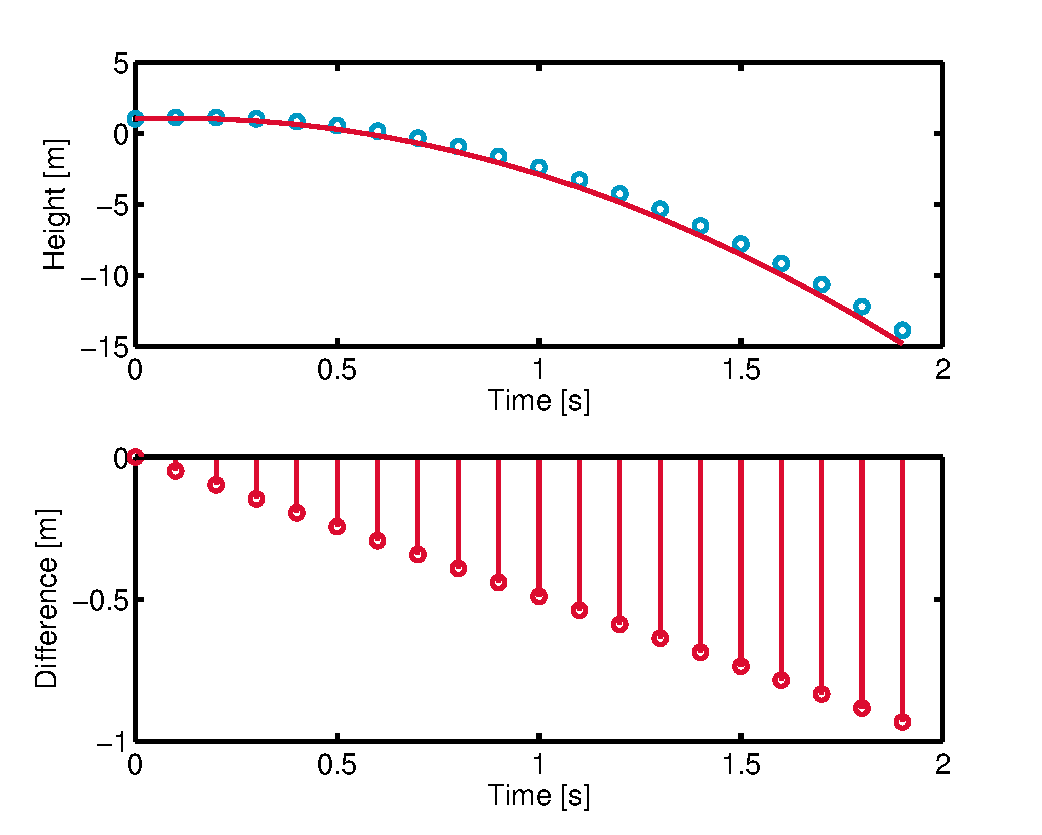
\includegraphics[width=0.8\textwidth]{projectile-utc}
%  \end{center}
%\end{frame}